\documentclass[10pt,a4paper]{labreport}
\usepackage{csquotes}
\usepackage{titlesec}
\usepackage{ragged2e}
\usepackage{siunitx}
\usepackage{setspace}
\usepackage{longtable}
\usepackage{rotating}
\usepackage{xurl}
\usepackage{physics}
\usepackage{caption}
\usepackage{wrapfig}
\usepackage{tabularray}
\usepackage{fancyhdr}
\usepackage{subcaption}
\usepackage{lscape}
\usepackage{tensor}
\usepackage{multirow}
\usepackage{chemformula}
\usepackage[gen]{eurosym}
\usepackage{float}
\usepackage{bm}
\usepackage{lipsum}
\usepackage{parskip}
\usepackage{booktabs}
\usepackage{enumerate}
\usepackage[justification=justified]{caption}
\usepackage[nottoc]{tocbibind}
\usepackage{color}
\usepackage{bm}
\usepackage{listings}
\definecolor{codegreen}{rgb}{0,0.6,0}
\definecolor{codegray}{rgb}{0.5,0.5,0.5}
\definecolor{codepurple}{rgb}{0.58,0,0.82}
\definecolor{backcolour}{rgb}{0.95,0.95,0.92}
\lstdefinestyle{mystyle}{
    backgroundcolor=\color{backcolour},   
    commentstyle=\color{codegreen},
    keywordstyle=\color{codepurple},
    numberstyle=\tiny\color{codegray},
   % stringstyle=\color{grey},
    basicstyle=\ttfamily\footnotesize,
    breakatwhitespace=false,         
    breaklines=true,                 
    captionpos=b,                    
    keepspaces=true,                 
    numbers=left,                    
    numbersep=5pt,                  
    showspaces=false,                
    showstringspaces=false,
    showtabs=false,                  
    tabsize=5
}
\lstset{style=mystyle}
\usepackage{hyperref}
 \usepackage[
backend=biber,
style=chem-acs,articletitle=true,doi=true]{biblatex}
\addbibresource{references.bib}






\title{Nanoscale Material Modeling
\\
\normalsize{Week 5}} % Main title and sub title. 

\author{Ilija A. Gjerapić, S4437586; \href{mailto:i.a.gjerapic@student.rug.nl}{i.a.gjerapic@student.rug.nl}; \href{https://github.com/igjerapic/nmm-week5/}{@github} } % Name, student number, email

\supervisors{prof. dr. A. Giuntoli, prof. dr. J. Slawinska}

\begin{document}

\maketitle
\tableofcontents



  

\thispagestyle{firststyle}
\newpage
\section{Assignment 1: What is a Particle?}

\subsection{Role of looping structure}
The looping structure is responsible for moving the two fullerene molecules in discrete steps of 0.3 \AA and 0.1 \AA for large and small distances, respectively. After the two fullerene molecules are moved closer together, the system is run under nvt ensemble at 300K for 2.5 ps with the positions and forces on each atom being sampled ever 0.25 ps. For each distance step, 20 iterations are conducted providing a total of 40 iterations. The LAMMPS code responsible for the larger steps is provided in Listing \ref{lst:ass1_loop_code}
\begin{lstlisting}[caption={The LAMMPS code for moving the two fullerne molecules closer together for larger distances in discrete steps of 0.3 \AA over 20 iterations. After the inital movement of atom posisitions, the system is run under nvt ensemble at 300K for 2.5 ps with the positions and force on each atom being sampled ever 0.25 ps. },
  label=lst:ass1_loop_code]
label           loop
variable        loop_count equal 20 
variable        a loop ${loop_count} # iterator ranging from 1 to 20, inclusive. 

variable        large_shift equal 0.3 # moves molecules towards each other by 2*shift
displace_atoms  c60a move ${large_shift} 0 0 units box 
displace_atoms  c60b move -${large_shift} 0 0 units box 

dump            2 all custom 500 lmp_data/dump.data${a} id type xu yu zu fx fy fz
dump_modify     2 sort id
run 5000
undump 2
next            a # goes to next a value, but stops after a=20. 
jump            SELF loop # jumps to the label "loop" at the start of this code block
\end{lstlisting}

\subsection{Extraction of Potential of Mean Force}
The force and potential energy between the two molecules was extracted using MDAnalsyis. To achieve this, the COM on each molecule and the total force on each molecule was determined for every sampled point in the simulation. The total force of a single molecule for each frame was then projected on the vector connecting the COMs of the two molecules. These steps are outlined in Listing \ref{lst:ass1_force_project}. Only the forces on a single molecule were calculated as the other molecule feels an equal and opposite reaction in accordance with Newtons Laws of motion. 
\begin{lstlisting}[language=Python,
                   label=lst:ass1_force_project,
                   caption={The python code used to extract the total force of a molecule projected onto the vector connecting the two COMs of the molecules. The molecules were identified using \texttt{u.atoms.fragments} to group atoms based on if they are reachable by transversing bonds.}
                  ]
# Loop over the frames and load the positions and forces
for i, traj in enumerate(u.trajectory):    
    c60a  = u.atoms.fragments[0]
    c60b = u.atoms.fragments[-1]

    c60a_forces[i] = sum(c60a.forces.copy())
    c60b_forces[i] = sum(c60b.forces.copy())
    c60a_COM[i] = c60a.center_of_mass()
    c60b_COM[i] = c60b.center_of_mass()

# vector pointing from c60a COM to c60b COM
vect_connect = c60a_COM - c60b_COM

# projection of forces on molecule a onto vector connecting of COMs for each distance
distances = np.linalg.norm(vect_connect, axis=1)
force_projection = np.einsum('ij,ij->i', c60a_forces, vect_connect ) / distances
  \end{lstlisting}

The calculated force projections were then averaged over 50 distance bins using the code outlined in Listing \ref{lst:ass1_force_averageing}.
\begin{lstlisting}[language=Python,
                   label=lst:ass1_force_averageing,
                   caption={The python code used to average out the force projections }
                  ]
# Setting up bins
min_dist = min(distances)
max_dist = max(distances)
num_bins = 50

bin_edges = np.linspace(min_dist, max_dist, num_bins)
bin_centers = 0.5 * (bin_edges[:-1] + bin_edges[1:])

# averaging forces on molecule A
avg_forces = np.zeros_like(bin_centers)
for i in range(len(bin_centers)):
    mask = (distances >= bin_edges[i]) & (distances <= bin_edges[i + 1])
    avg_forces[i] = np.average(force_projection[mask])

# removing nan values
valid_indices = ~np.isnan(avg_forces)
avg_forces_valid = avg_forces[valid_indices]
bin_centers_valid= bin_centers[valid_indices]
\end{lstlisting}
The potential energy was then extracted from these forces:
\begin{equation}
  V = - \int_O^\infty \vb{F} \cdot \vb{d}r = \int_\infty^O \vb{F} \cdot \vb{d}r
\end{equation}
using the \texttt{scipy.integrate.trapezoid} method as shown in Listing \ref{lst:ass1_PMF}
\begin{lstlisting}[language=Python,
                   label=lst:ass1_PMF,
                   caption={The python code used to determine the PFM. Integration starts from larger distances to smaller to allow for complete integration of the forces. Actual itegration is achieved using the \texttt{scipy.integrate.trapezoid} function.}
                  ]
# determining Potential Mean Field 
potential= np.zeros(len(bin_centers_valid))
for i in range(len(bin_centers_valid) - 1, 0, -1):
    potential[i-1] = potential[i] + trapezoid(avg_forces_valid[i-1:i+1], 
                                          x= bin_centers_valid[i-1:i+1] )
\end{lstlisting}

\subsection{Course Graining}
The extracted mean force and potential of mean force is shown in Figure \ref{fig:ass1_force-and-PMF}(a) and Figure \ref{fig:ass1_force-and-PMF}(b), respectively. 
The Lennard-Jones potential
\begin{equation}
  V_\text{LJ} = 4 \epsilon \left[ \left(\frac{\sigma}{r}\right)^{12} - \left(\frac{\sigma}{r}\right)^{6}\right],
\end{equation}
where $\epsilon$ is the well depth, and $sigma$ the zero-crossing distance
along with the Morse potential
\begin{equation}
  V_\text{Morse} = D_e\left( e ^{-2 a (r- r_0)} - 2 e^{-a(r-r_0)}\right),~~ a = \sqrt{\frac{k}{2D_e}},
\end{equation}
were $D_e$ is the well depth, $k$ the force constant of the bond, and $r_0$ the equilibirium bond distance were fitted to the PMF as shown in Figure \ref{fig:ass1_force-and-PMF}(b). The non-bonded interactions are best described with a Morse potential. 
\begin{figure}[h!]
  \centering
  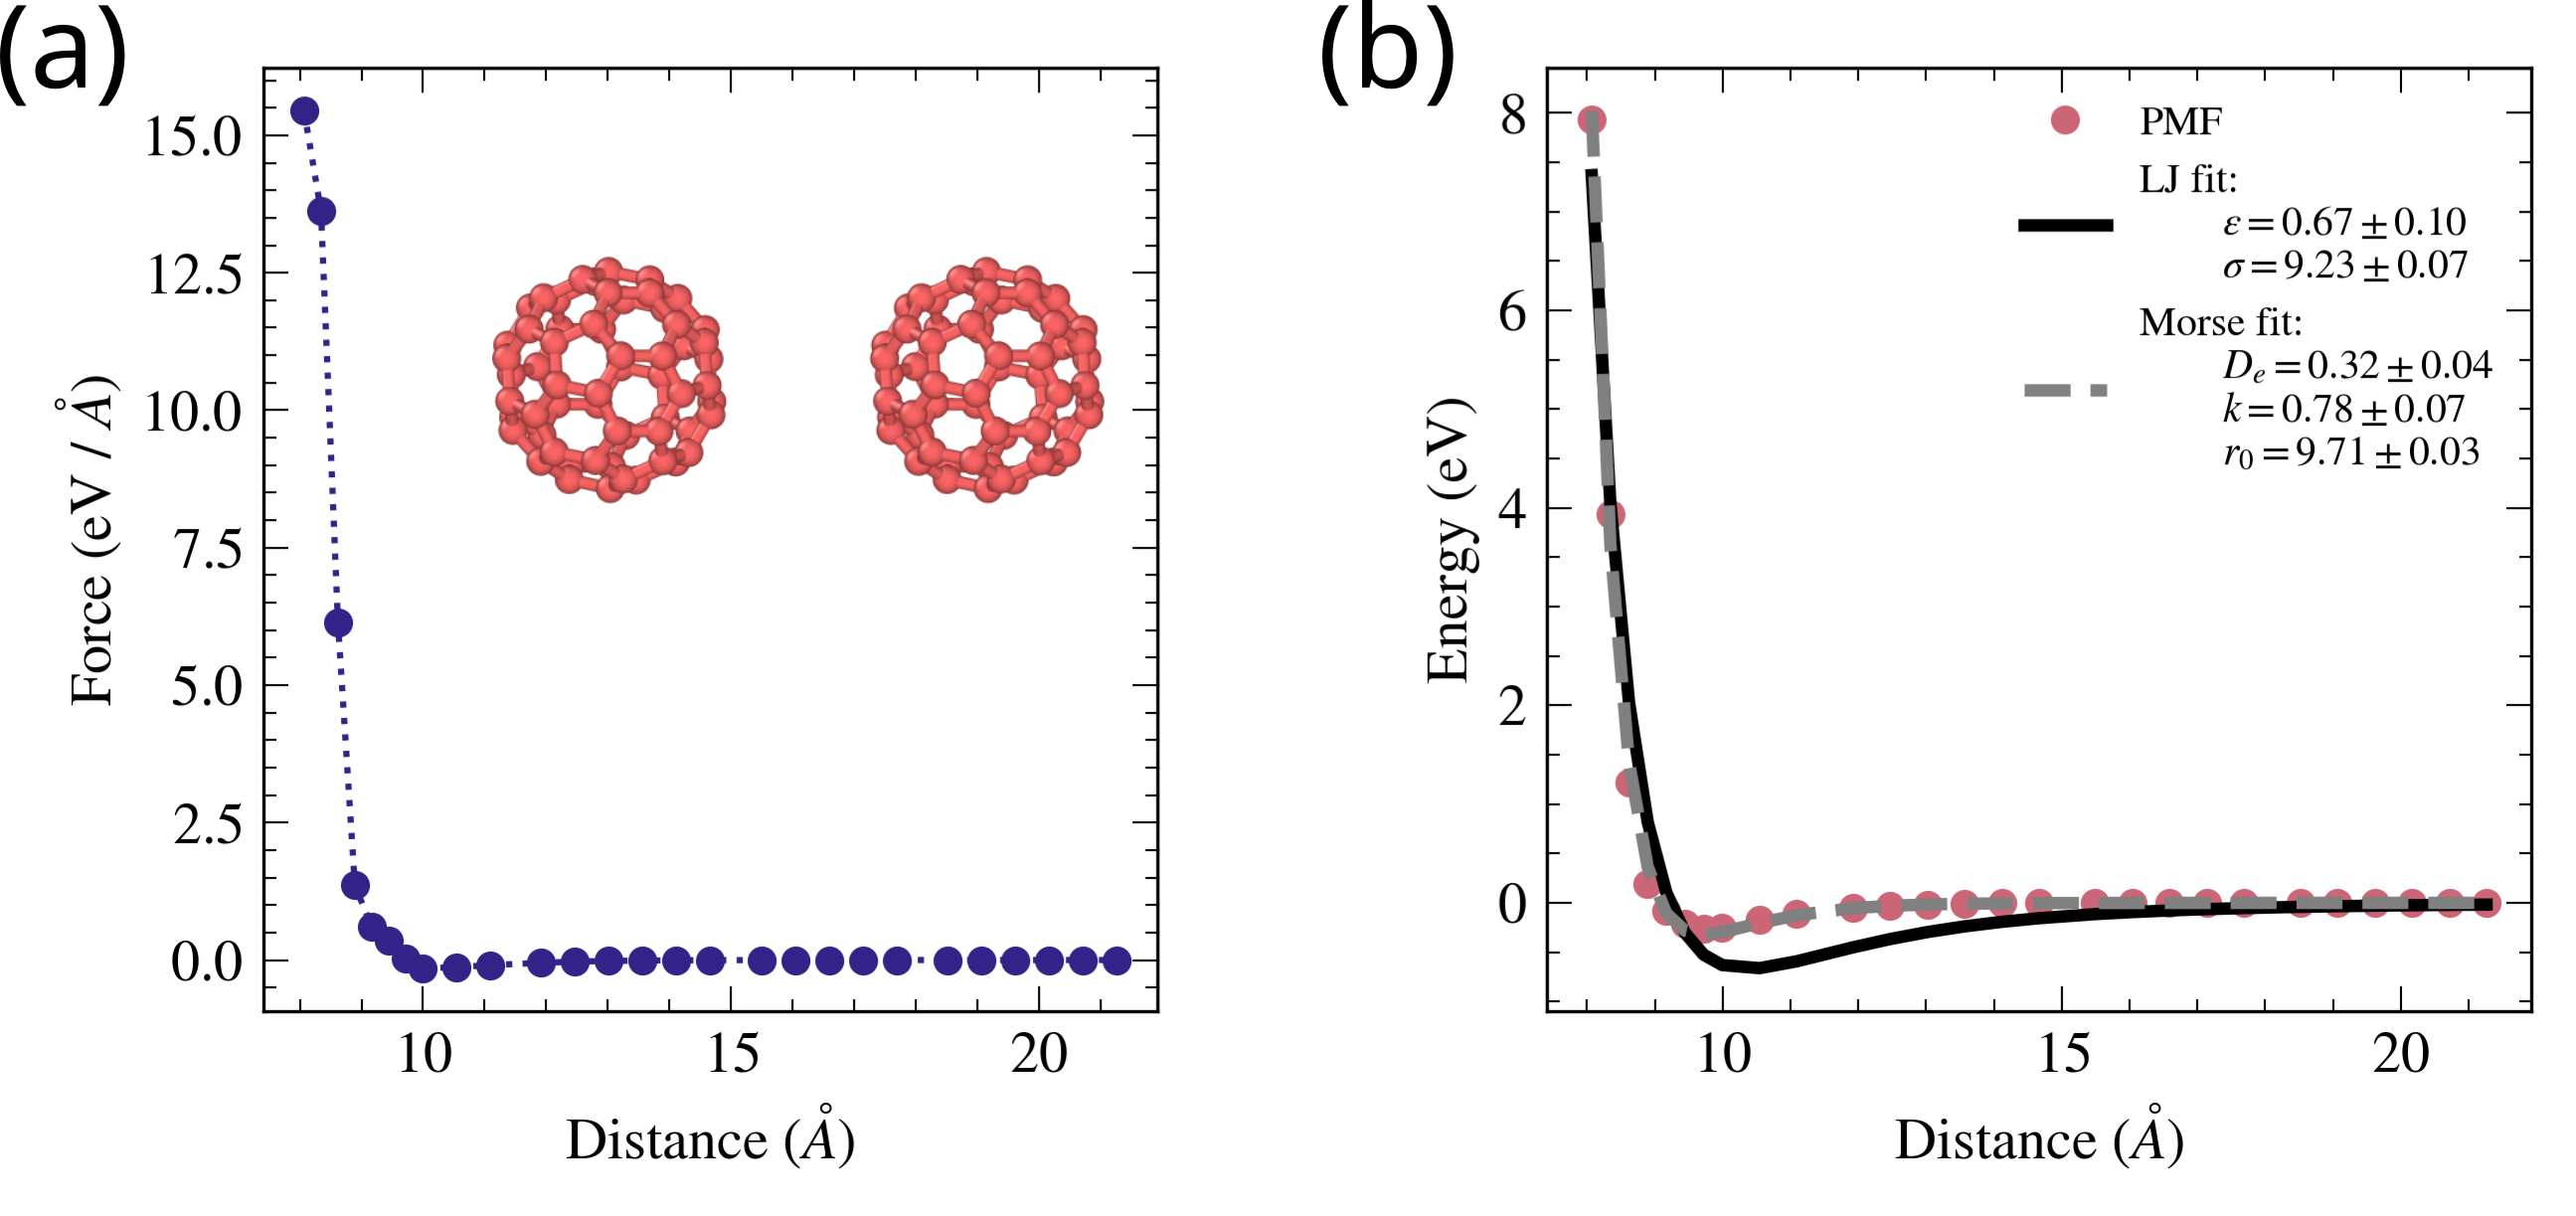
\includegraphics[width = 0.8\textwidth]{figs/ass1.png}
  \caption{The averaged force (a) and the potential of the mean force (b) calculated for two fullerene molecules. The Lennard-Jones (black solid line) and the Morse (grey dashed line) potentials were fitted to the PMF using \texttt{scipy.optimize.curve\_fit}. The Morse potential most accurately describes the PMF. The inset of (a) is an \texttt{ovito} snapshot of the two fullerene molecules.}
  \label{fig:ass1_force-and-PMF}
\end{figure}

A simulation utilizing the coarse-grained particles would require the mass, the fitting parameters, and the diameter of the particles. 
For the case of fullerene, the mass is 750 g/mol, the diameter 7.1 \AA (determined from the average $R_g$ from the previous simulations), and the fitting parameters are shown in Figure \ref{fig:ass1_force-and-PMF}. 
An implementation of these course-grained particles is shown in Listing \ref{lst:ass1_CG}.
The difference between a CG particle and an all-atom fullerene is showed in Figure \ref{fig:ass1_CG}(a), while the result of Listing \ref{lst:ass1_CG} is showed in Figure \ref{fig:ass1_CG}(b).  

\begin{lstlisting}[
                  label=lst:ass1_CG,
                  caption={An example implementation of the start of a simulation of our coarse-grained  fullerene molecules. The result is seen in Figure \ref{fig:ass1_CG}(b).}
]
dimension     3
units         metal
atom_style    full
boundary      p p p

# Variables
variable      N equal 200    # number of particles   
variable      eta equal 0.3   # packing fraction    
variable      temp equal 300.0  # temperature

variable      sigma equal 7.1     # diameter from avg R_g of one molecule
variable      particle_volume equal (4.0/3.0)*PI*(0.5*${sigma})^3  
variable      total_volume equal ${N}*${particle_volume}
variable      lbox equal (${total_volume}/${eta})^(1.0/3.0) 
variable      l equal 0.5*${lbox}
variable      rand_seed equal 5468945

region        box block -${l} ${l} -${l} ${l} -${l} ${l}
create_box    1 box
create_atoms  1 random ${N} ${rand_seed} box

mass          1 750
pair_style    morse     17.5
pair_coeff    1 1 0.32  1.104  9.71  # D_e,  a,  r_0 

minimize      0.0 1.0e-8 1000 100000

write_data    relaxed_CG.data
\end{lstlisting}
\begin{figure}[h!]
  \centering
  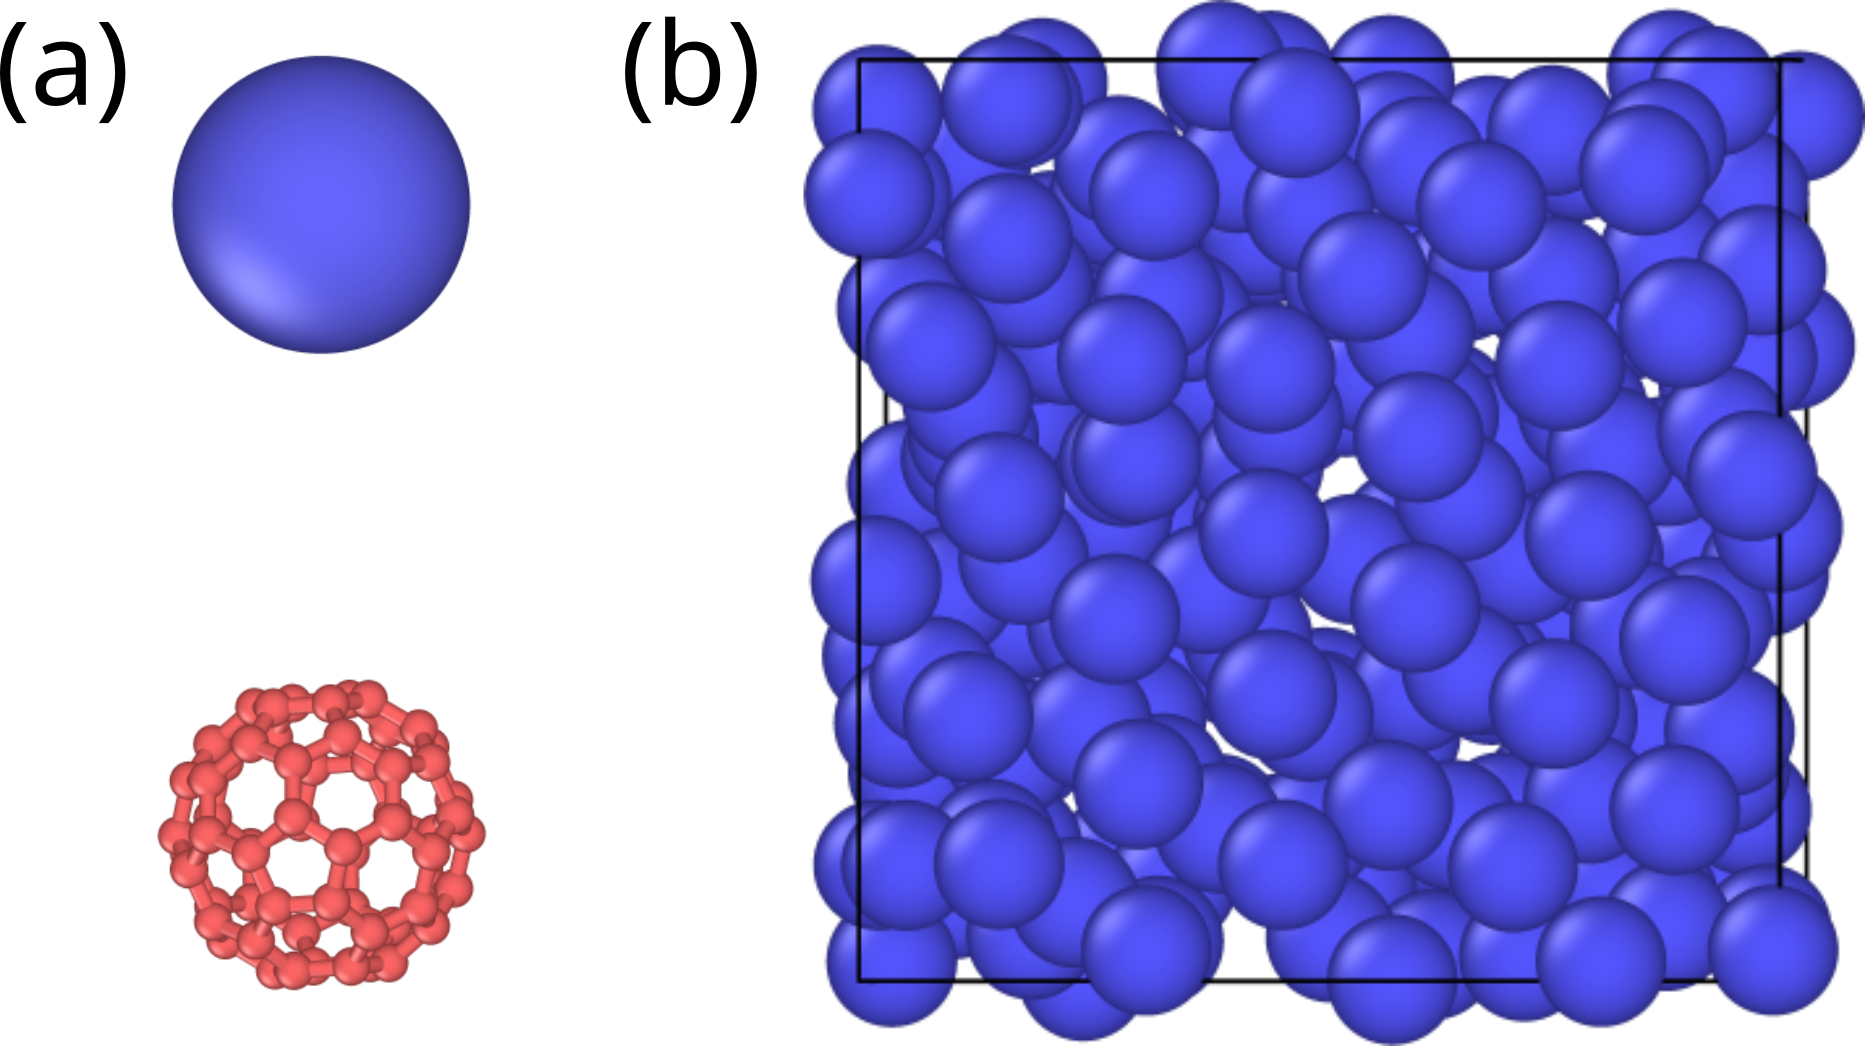
\includegraphics[width = 0.6\textwidth]{figs/ass1_CG.png}
  \caption{(a) The comparison between an all-atom fullerene molecule and its coarse-grained bead, from \texttt{fullerene\_CG.data}. (b) The result of the 200 coarse-grained fullerene beads in a 30 v\% box.}
  \label{fig:ass1_CG}
\end{figure}

\newpage
\section{Assignment 2: Just Jamming}
The input script was adjusted such that the packing fraction $\eta$ and the interaction strength $\epsilon$ could be inputted as variables using \texttt{lmp -in in.3dlj -v ETA \$eta -v EPSILON \$epsilon}. 
\begin{lstlisting}
# Variables
variable 	    N equal 2048      # number of particles   
variable 	    eta equal ${ETA}  # packing fraction     
variable 	    temp equal 1.0    # temperature
variable      epsilon equal ${EPSILON}

# ...

pair_style	  lj/cut 2.5
pair_coeff	  1 1 ${epsilon} 1.0 2.5 
\end{lstlisting}

For a fixed packing fraction of $\eta = 0.4$, the interaction strength was varied to be $\epsilon\in\{0.5, 0.2, 5.0\}$. All simulations reached equilibrium as shown in Figure \ref{fig:ass2_thermos_eta0.4}. 
\begin{figure}[h]
  \centering
  \includegraphics[width = 1.0\textwidth]{figs/eta0.4_thermos.png}
  \caption{The (a) temperature, (b) pressure and (c) total energy against the simulation time for a LJ substance with packing fraction of $\bm{\eta = 0.4}$ and interaction strengths $\bm{\epsilon = 0.5} \text{ (red), } \bm{2.0} \text{ (dark blue), } \bm{5.0}\text{ (light blue)}$. The plateaus in all thermodynamic properties demonstrate that each simulation reached equilibrium.}
  \label{fig:ass2_thermos_eta0.4}
\end{figure}

Figure \ref{fig:ass2_rdf-msd_eta0.4} shows the radial distribution function and the mean square displacement (MSD) for an LJ substance with a packing fraction of 0.4.
For interaction strengths of 0.5 and 2.0, the LJ substance is a liquid, while the LJ substance is crystalline with $\epsilon = 5.0$. 
The liquid behavior is supported by the less intense and broad peaks that quickly decay in the RDF. 
For the crystalline phase with $\epsilon=0.5$, the peaks in the RDF are much more intense and sharper. Moreover, the MSDs for $\epsilon = 0.5,2.0$ both show  a ballistic region followed by diffusion. 
The crystalline phase of $epislon=0.5$ is supported by the plateau in the MSD after 10$^2$ $\tau$. 
\begin{figure}[htbp]
  \centering
  \includegraphics[width = 0.95\textwidth]{figs/eta0.4_rdf-msd.png}
  \caption{The (a) RDF and (b) MSD for a LJ substance with packing fraction of $\bm{\eta = 0.4}$ and interaction strengths $\bm{\epsilon = 0.5} \text{ (red), } \bm{2.0} \text{ (dark blue), } \bm{5.0}\text{ (light blue)}$. For interaction strengths of 0.5, 0.2 the LJ substance is a liquid, but is crystalline for an interaction strength of 5.0.}
  \label{fig:ass2_rdf-msd_eta0.4}
\end{figure}

The crystalline phase for $eta=0.4, \epsilon=5.0$ and liquid phases for $eta = 0.4, \epsilon=0.2,0.5$ are qualitatively confirmed by using the \texttt{common neighbor analysis} modification in \texttt{ovito} as shown in Figure \ref{fig:ass2_common_eta0.4}. This shows that the crystalline structure is primarily FCC, with some HPC contributions. 
\begin{figure}[htbp]
  \centering
  \includegraphics[width = 0.95\textwidth]{figs/eta0.4_common.png}
  \caption{The \texttt{common neighbor analysis} for the final configuration for an LJ substance at temperature 1.0 with a packing fraction 0.4 and interaction strength (a) $\bm{\epsilon=0.5}$, (b) $\bm{\epsilon=2.0}$ (c) $\bm{\epsilon=5.0}$. The LJ substance forms a crystalline structure of mixed HPC and FCC packing for an interaction strength of 5.0, while for interaction strengths of 0.5 and 2.0, no crystalline structures are observed. }
  \label{fig:ass2_common_eta0.4}
\end{figure} 

\newpage
\section{Assignment 3: Patch up}
Two initial data files with patchy particles were built with one consisting of 25\% particles having 2 patches ($N_2$) and 75\% having 4 patches ($N_4$) and the other having equal number of $N_2$ and $N_4$ particles. The naming convention for each system is $N_2\_Y$, where $Y$ is the fraction of particles that are $N_2$. 
Figure \ref{fig:ass3_patchy_particles} shows the visualization of the two different patchy particles considered.
\begin{figure}[h]
  \centering
  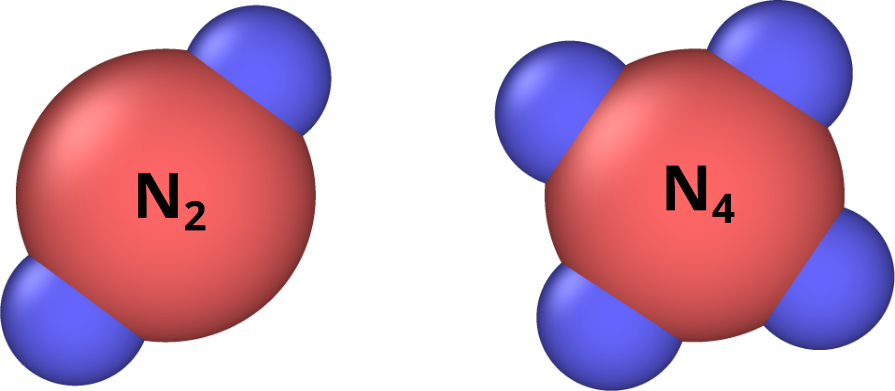
\includegraphics[width = 0.5\textwidth]{figs/ass3_particles.png}
  \caption{\texttt{Ovito} images of the patchy particles considered.}
  \label{fig:ass3_patchy_particles}
\end{figure}



Each system has a volume fraction $\phi=0.2$ following \cite{zhangSelfAssemblyPatchyParticles2004}. Moreover, for each system, the simulation was run at a temperature of $T=0.5$ and $T=2.0$. The lower bound was chosen as Zhang \textit{et al.}, showed that $N_4$-like particles form sheets below $k_BT/\epsilon = 1.0$, while $N_2$-like particles form long chains at  $k_BT/\epsilon = 0.5$.  On the other hand, Zhang \textit{et al.} showed $N_4$ particles form a disordered state above $k_BT/\epsilon = 1.67$ and $N_2$ above $k_BT/\epsilon = 1.67$ \cite{zhangSelfAssemblyPatchyParticles2004}. 
The evidence that each system reached equilibrium before analyzing the final frame is shown in Figure \ref{fig:ass3_Nx0.25_thermos} and Figure \ref{fig:ass3_Nx0.5_thermos} for $N_2\_0.25$ and $N_2\_ 0.5$, respectively. 

\begin{figure}[htbp]
  \centering
  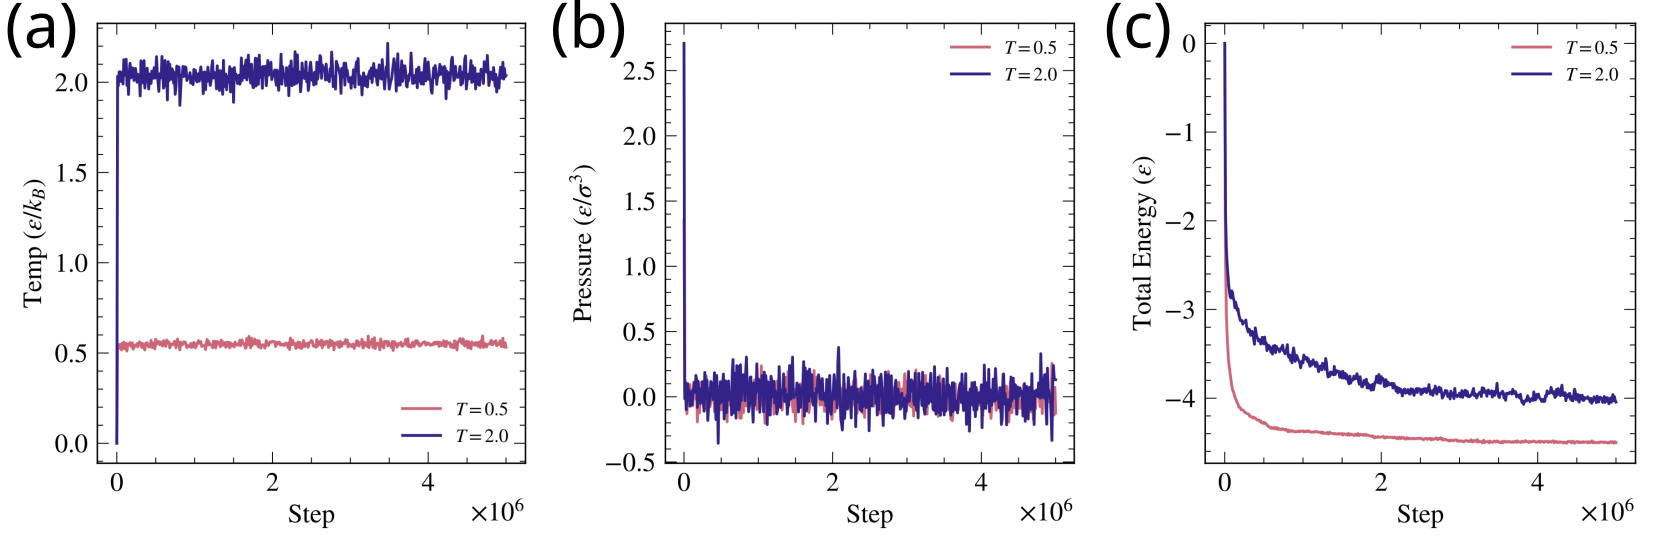
\includegraphics[width = 0.95\textwidth]{figs/ass3_Nx0.25_thermos.png}
  \caption{The thermodynamic properties (a) temperature, (b) pressure and (c) Total energy of the $\bm{N_2\_ 0.25}$ system overtime at $\bm{k_BT / \epsilon = 0.5}$ (red) and $\bm{k_BT/\epsilon = 2.0}$ (blue). } 
  \label{fig:ass3_Nx0.25_thermos}
\end{figure}


The results of the simulations are shown in Figure \ref{fig:ass3_results}(a-d). 
In all systems clusters of atoms are formed, but of different sizes and general shapes. 

To quantitatively characterize the size of the clusters formed, the number of constitute atoms is considered. 
To avoid clusters consisting of only two patchy particles, a cluster is considered to be formed when more than eight atoms can be traversed with a cutoff distance of 1.5. 
This results in the smallest clusters consisting of three patchy particles as $N_2$ and $N_4$ consist of three and five atoms, respectively. The final ensemble averaged cluster size for each system is show in Figure \ref{fig:ass3_results}(e).

The shape of the cluster is quantified by the "acircularity" $c$,
\begin{equation}
  c = \lambda_1 ^2 - \lambda_2^2,~~ \lambda_1 > \lambda_2,
\end{equation}
where $\lambda_{1,2}$ are the eigenvalues of the 2D gyration tensor. 
The acircularity is my 2D analog to the acylindricity. 
The acircularity of a cluster is exactly zero if the particles are homogeneously distributed in the x-y plane (e.g square or circular sheets), and gives higher values for more linear clusters. A comparison of the final ensemble averaged acircularity for each system is shown in Figure \ref{fig:ass3_results}(f)

For both system compositions, larger chain-like clusters are formed at $k_BT / \epsilon = 0.5$, while smaller sheet clusters are formed at  $k_BT / \epsilon = 2.0$. 

\begin{figure}[p]
  \centering
  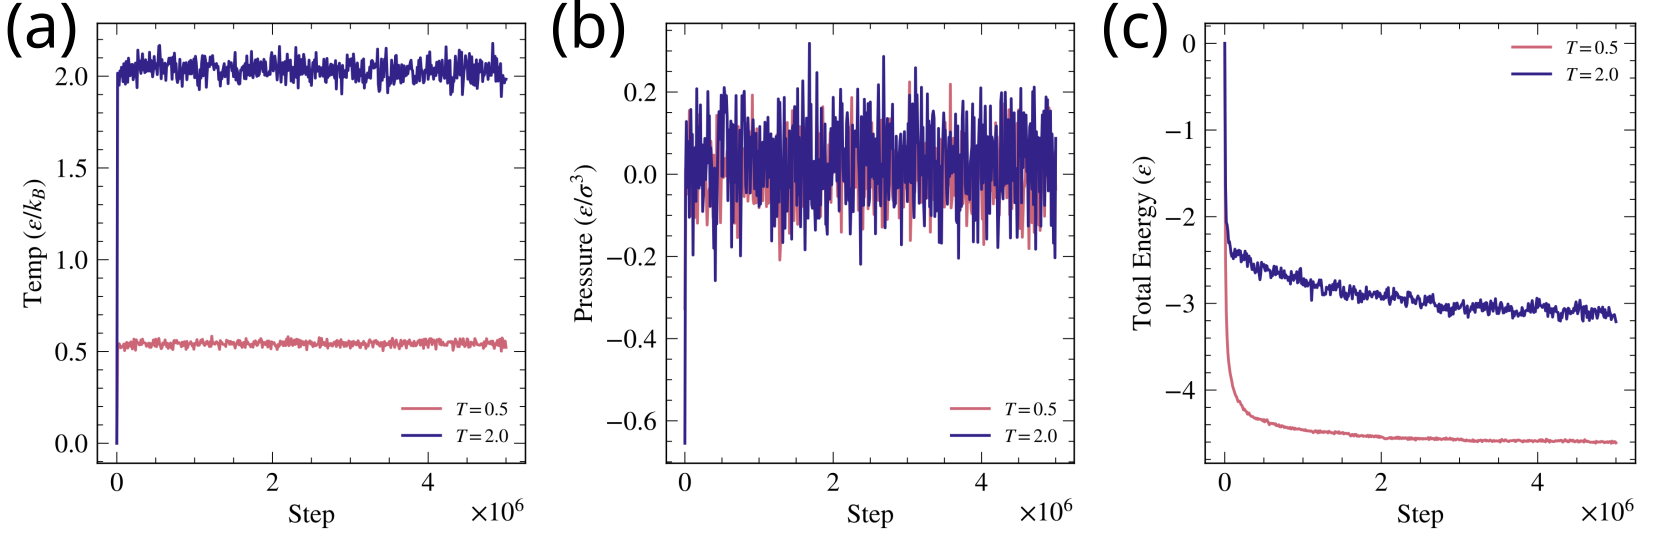
\includegraphics[width = 0.95\textwidth]{figs/ass3_Nx0.5_thermos.png}
  \caption{The thermodynamic properties (a) temperature, (b) pressure and (c) Total energy of the $\bm{N_2\_ 0.5}$ system overtime at $\bm{k_BT / \epsilon = 0.5}$ (red) and $\bm{k_BT/\epsilon = 2.0}$ (blue). } 
  \label{fig:ass3_Nx0.5_thermos}
\end{figure}
\begin{figure}[p]
  \centering
  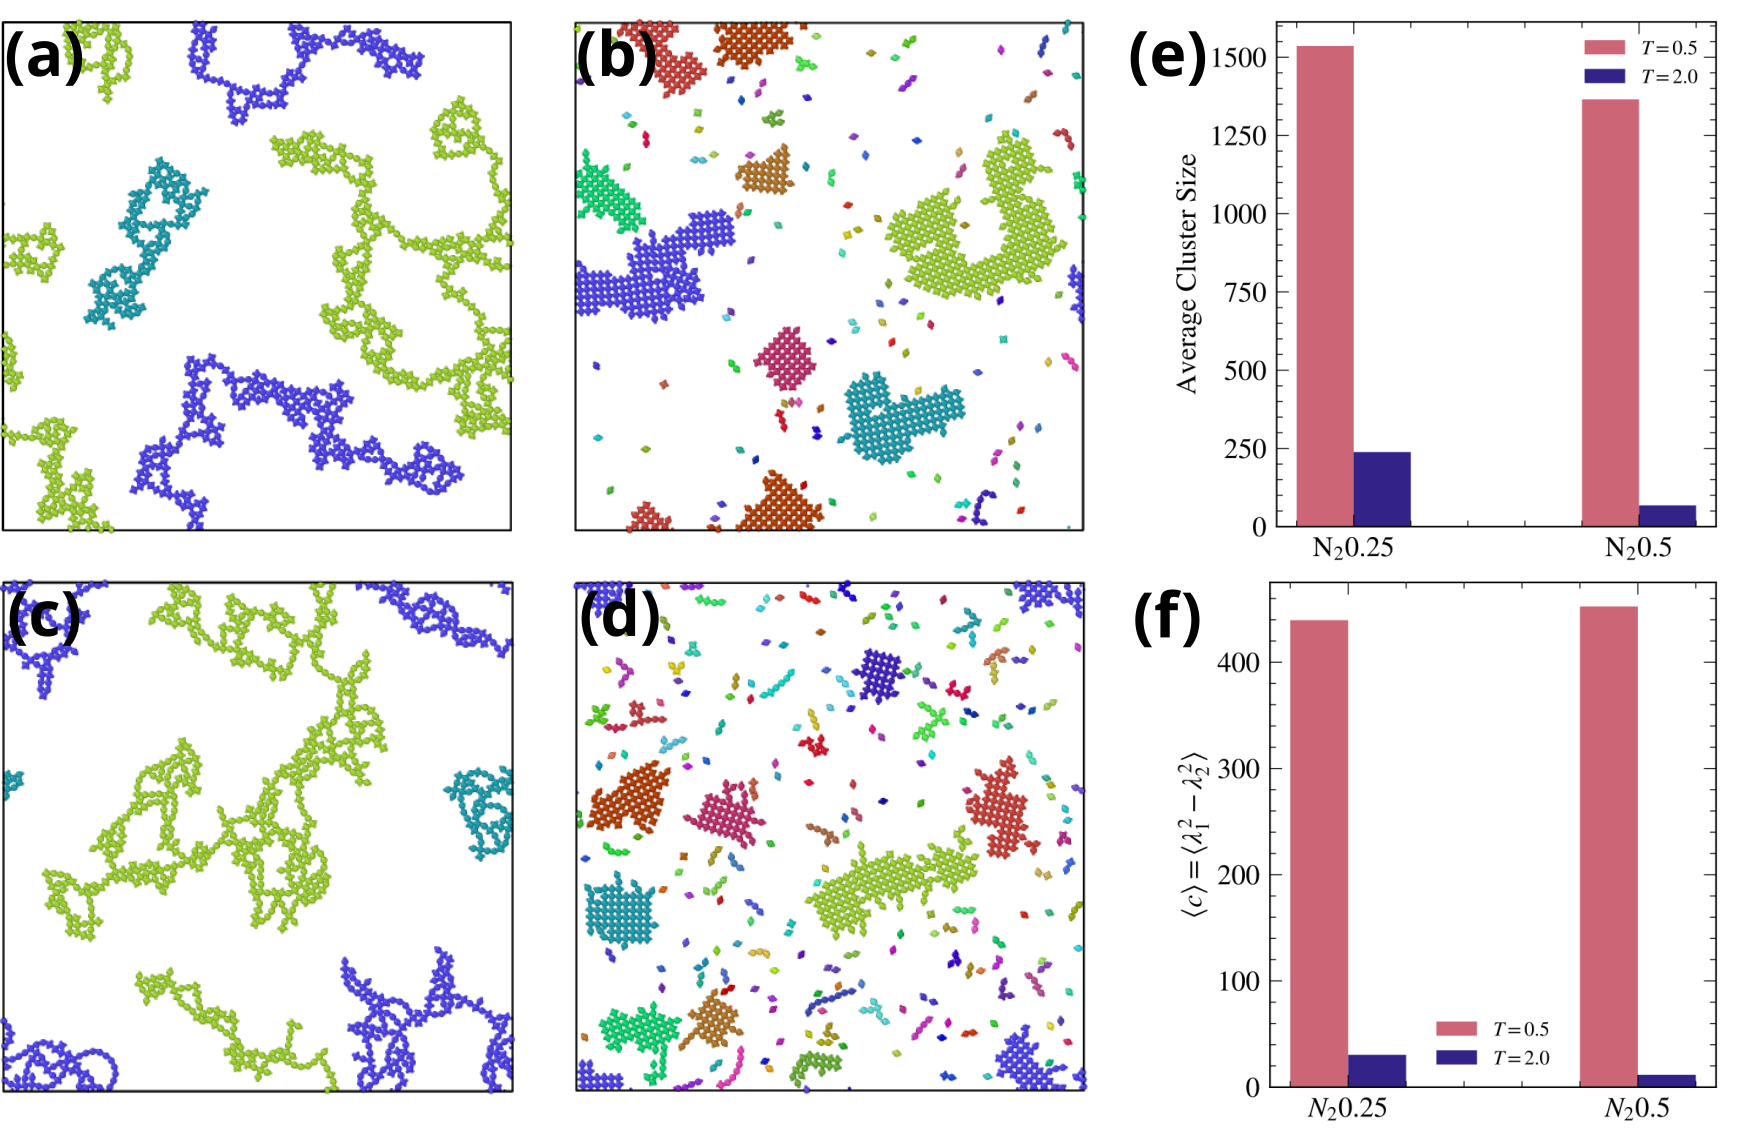
\includegraphics[width = \textwidth]{figs/ass3_results.png}
  \caption{The final configurations of (a) $\bm{N_2\_0.25}$ $\bm{k_BT / \epsilon = 0.5}$, (b)  $\bm{N_2\_0.25}$ $\bm{k_BT / \epsilon = 2.0}$,  (c) $\bm{N_2\_0.5}$ $\bm{k_BT / \epsilon = 0.5}$ and (d) $\bm{N_2\_0.5}$ $\bm{k_BT / \epsilon = 2.0}$. The atoms are colored by their cluster, defined by a cutoff distance of 1.5. (e) The cluster size characterized by the number of constituent atoms. A cluster is considered to be formed when a cluster consists of more than eight atoms. (f) The shape of the clusters is characterized by the average "acircularity", $\bm{c = \lambda_1^2 - \lambda_2^2}, ~ \lambda_1 > \lambda_2$. For both compositions, larger chain-like clusters are formed at the lower temperature, while smaller sheets are formed at the higher temperature.} 
  \label{fig:ass3_results}
\end{figure}

\newpage
\section{Assignment 4: Look Ma, no hands!}
The temperature is stabilized using the \texttt{fix nvt/sllod} command. 
This command performs a constant NVT integration to update the atom positions and velocities for a simulation box that is changing size and/or shape. 
The NVT ensemble is implemented using the Nos\'{e}-Hoover temperature thermostat, which globally rescales the kinetic-energy of the particles such that the Nos\'{e}-Hoover non-Hamiltonian is conserved \cite{frenkelUnderstandingMolecularSimulation2023}. 
In our case, the global kinetic-energy is rescaled every 100 time steps. 

To determine the flow-curve of colloids, the equilibrated structure of an LJ substance at temperature 1.0, packing fraction 0.58, $\epsilon = 1.0$ was subjected to shear rates of $\dot{\gamma} \in \{0.001, 0.005, 0.01, 0.05, 0.1, 0.2, 0.4, 0.5, 0.8, 1.0\}$.
Figure \ref{fig:ass4_equilib} shows the initial configuration was in equilibrium before the shear was applied. 
\begin{figure}[h!]
  \centering
  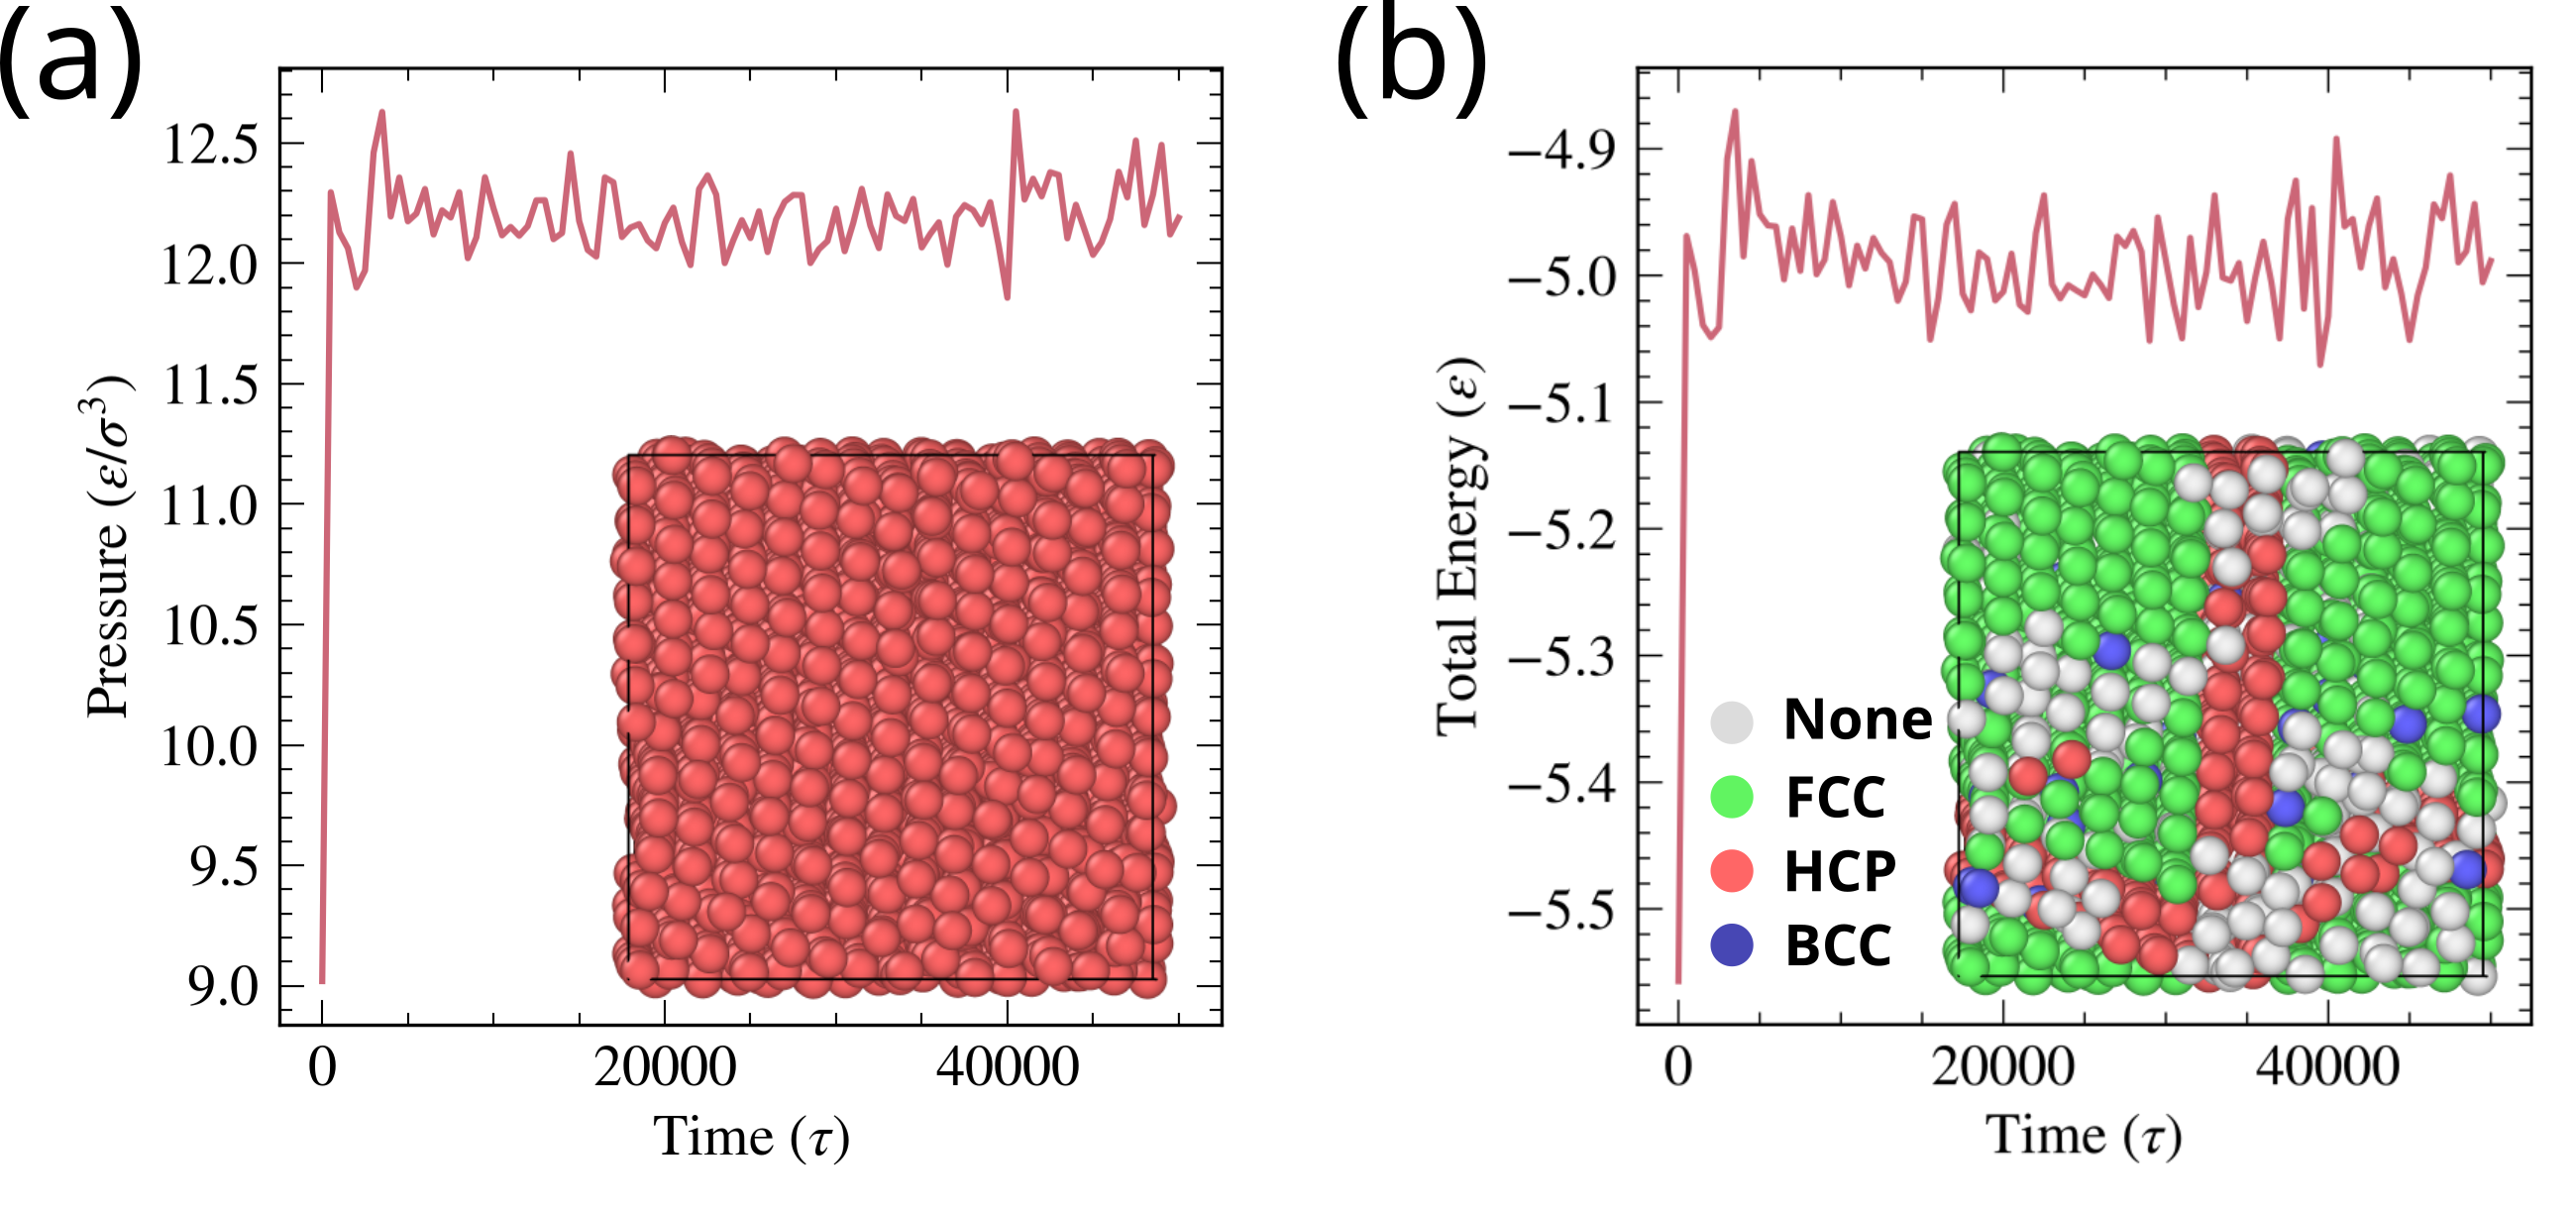
\includegraphics[width = 0.95\textwidth]{figs/ass4_equilib.png}
  \caption{The time evolution of the (a) pressure and (b) total energy for the LJ substance with a packing fraction of 0.58 and interaction energy 1.0 at temperature 1.0. The inset in (a) shows the final configuration of the substance and the inset in (b) shows the same configuration but colored according to the \texttt{common neighbor analyis} by \texttt{ovito}. The final configuration was used before applying different shear rates.}
  \label{fig:ass4_equilib}
\end{figure}

The viscosity was determined from the stress-strain curves. 
To determine the stress of the system due to the strain, the stress per atom was first calculated. 
The total stress was then computed as the sum of the xy component of the stress/atom  over all atoms. The computed stress is given in units of pressure*volume, thus it is multiplied by the total particle volume. 
The implementation using LAMMPS is shown in Listing \ref{lst:ass4_stress_compute}.
\begin{lstlisting}[
                    label=lst:ass4_stress_compute,
                    caption={The LAMMPS lines used to calculate the stress of the system.}
                  ]
compute     stressA all stress/atom NULL   # given in pressure*volume units 
compute     s4 all reduce sum c_stressA[4] # 4th element is xy component
\end{lstlisting}
The resulting stress-strain curves for the varius strain rates are shown in Figure \ref{}(a). 
Further observation shows that for every strain rate, a steady-flow is obtained after a strain of 1\%.
Thus, the mean steady-state stress $\langle \sigma \rangle$ is given by the average of the stresses for strains of 1\% and higher.
The corresponding viscosity is given by 
\begin{equation}
\eta = \langle \sigma \rangle / \dot\gamma,
\end{equation}
where $\dot{\gamma}$ is the shear rate. 
The resulting flow curve is shown in Figure \ref{fig:ass4_flows}. 
A power law fit results in an exponent of $-0.96 pm 0.01$. 
A lower bound for the zero-shear viscosity is conservatively estimated to be $0.7 \epsilon \tau / \sigma ^3$ by taking the average of the viscosities corresponding to the two lowest shear rates.
\begin{figure}[h!]
  \centering
  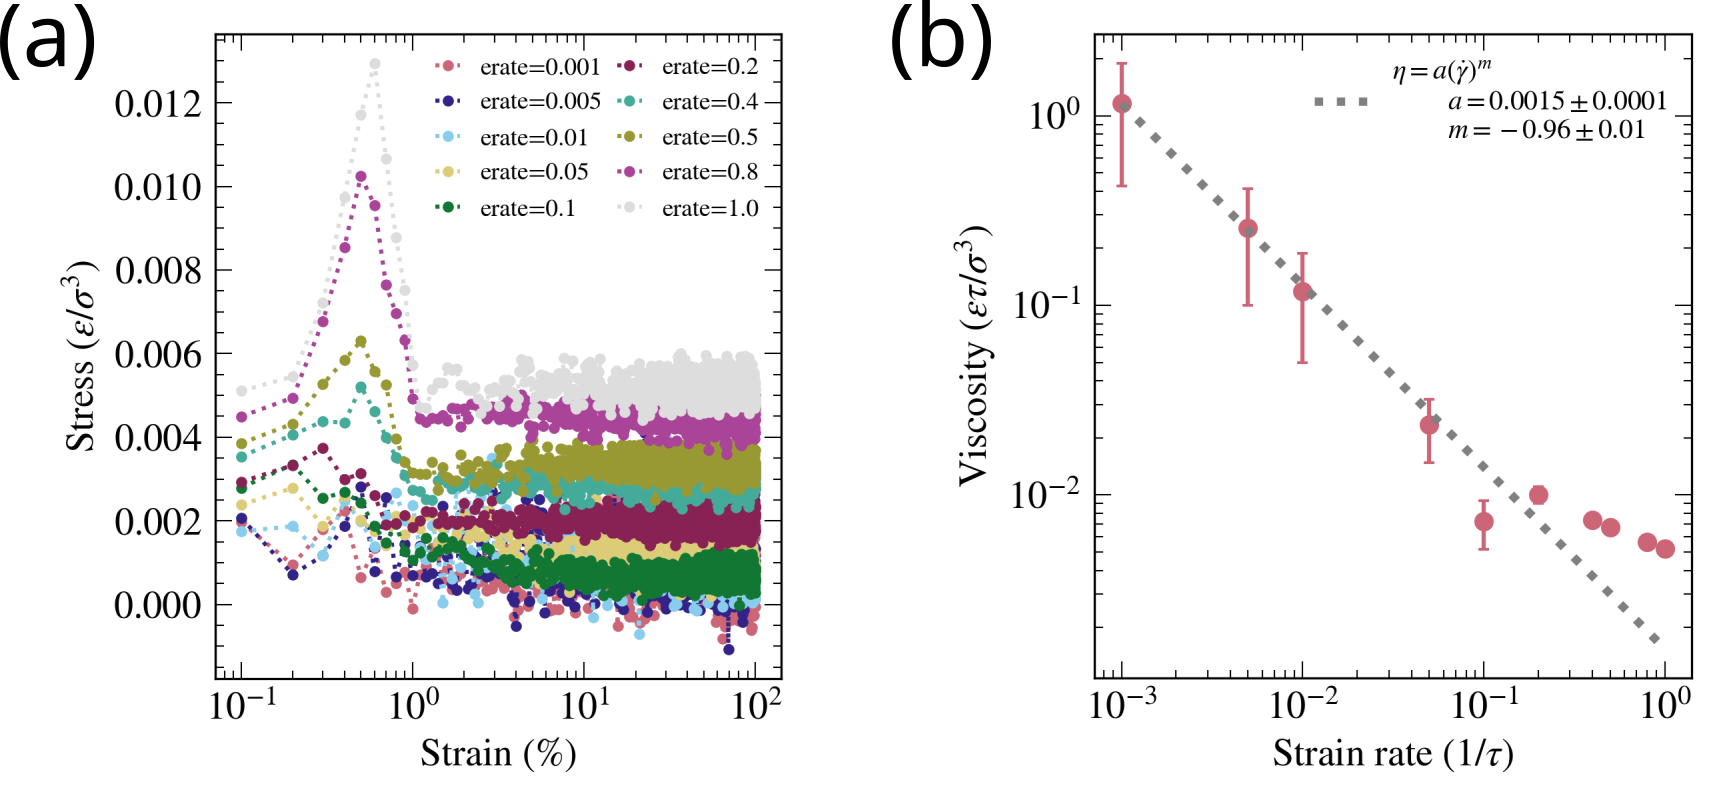
\includegraphics[width = 0.95\textwidth]{figs/ass4_strain.png}
  \caption{(a) The stress-strain curves for all strain-rates $\bm{\dot{\gamma}}$ considered. For all strain-rates, a steady-flow is obtained after a strain of 1\%. (b) The flow curve obtained by taking the viscosity $\eta$ as the mean steady-state stress divided by the corresponding shear rate. The mean steady-state stress was determined as the average of the stresses for strains larger than 1\%. A power law (grey dashed line) was fit with relative success. A lower bound of the zero-shear viscosity is determined to be $\bm{0.7 \epsilon \tau / \sigma ^3}$ from the average of the two lowest shear-rates. }
  \label{fig:ass4_flows}
\end{figure}






  % \begin{table}[h]
  %   \caption{An overview of the number of each bond type for the output files considered.}
  %   \label{tab:ass1_lammps-bonds}
  %   \centering
  %   \begin{tabular}{cccc}
  %     \hline
  %   \textbf{Bond Type}      & \textbf{No-reacted}     & \textbf{Half-reacted}   & \textbf{Full-reacted}   \\
  %   \hline
  %   1 & 216000 & 216000 & 216000 \\
  %   2 & 0      & 10947  & 18861  \\
  %   3 & 0      & 0      & 0      \\
  %   4 & 0      & 0      & 0      \\ \hline
  %   \textbf{Total} & 216000 & 226947 & 234861 \\ \hline
  %   \end{tabular}
  % \end{table}
  % \begin{figure}[h]
  %   \centering 
  %   \includegraphics[width = 0.7\textwidth]{figs/ass1_Si_cryst.png}
  %   \caption{\textbf{(a)} The conventional FCC unit cell with a two atom basis. The lattice constant was found to be 5.43 \AA. with a bond angle of 90$^\circ$. (b) The primitive unit cell obtained from the input file. A lattice constant of 3.8396 {\AA} was found, with a bond angle of 60$^\circ$.}
  %   \label{fig:ass1_cryst}
  % \end{figure}
  
\newpage 
\printbibliography

\end{document}



